% =============================================================================
%  Ratatouille: Capstone Project Report
%  Nindra Dhanush (MT25074) | CoSyLab, IIIT Delhi
%  Supervisor: Prof. Ganesh Bagler | July 2026
% =============================================================================
%  Compile with: pdflatex Ratatouille_Report.tex  (run twice for TOC/refs)
%  Or:           xelatex  Ratatouille_Report.tex
% =============================================================================

\documentclass[12pt, a4paper]{article}

% ---------- packages ----------
\usepackage[a4paper, top=2.5cm, bottom=2.5cm, left=2.8cm, right=2.8cm]{geometry}
\usepackage{fontenc}
\usepackage[utf8]{inputenc}
\usepackage{lmodern}
\usepackage{microtype}
\usepackage{setspace}
\usepackage{parskip}
\usepackage{titlesec}
\usepackage{titletoc}
\usepackage{fancyhdr}
\usepackage{graphicx}
\usepackage{amsmath, amssymb}
\usepackage{mathtools}
\usepackage{booktabs}
\usepackage{longtable}
\usepackage{array}
\usepackage{tabularx}
\usepackage{multirow}
\usepackage[table,xcdraw]{xcolor}
\usepackage{listings}
\usepackage{lstautogobble}
\usepackage{mdframed}
\usepackage{enumitem}
\usepackage{hyperref}
\usepackage{cleveref}
\usepackage{caption}
\usepackage{float}
\usepackage{tikz}
\usetikzlibrary{shapes.geometric, arrows, positioning, calc}
\usepackage[normalem]{ulem}
\usepackage{soul}

% ---------- colours ----------
\definecolor{iitdblue}{RGB}{0, 56, 116}
\definecolor{iitdgold}{RGB}{180, 141, 50}
\definecolor{codebg}{RGB}{248, 248, 248}
\definecolor{codeframe}{RGB}{200, 200, 200}
\definecolor{keywordcolor}{RGB}{0, 100, 180}
\definecolor{commentcolor}{RGB}{100, 130, 100}
\definecolor{stringcolor}{RGB}{163, 21, 21}
\definecolor{highlightblue}{RGB}{230, 242, 255}

% ---------- hyperref ----------
\hypersetup{
    colorlinks   = true,
    linkcolor    = iitdblue,
    citecolor    = iitdblue,
    urlcolor     = iitdblue,
    pdftitle     = {Ratatouille: AI-Powered Cost-Constrained Indian Budget Recipe Generation},
    pdfauthor    = {Nindra Dhanush},
    pdfsubject   = {Capstone Project Report -- IIIT Delhi},
    pdfkeywords  = {Recipe Generation, LLM, Linear Programming, Vegan Substitution, NLP}
}

% ---------- listings (code) ----------
\lstset{
    backgroundcolor = \color{codebg},
    frame           = single,
    rulecolor       = \color{codeframe},
    basicstyle      = \ttfamily\small,
    keywordstyle    = \color{keywordcolor}\bfseries,
    commentstyle    = \color{commentcolor}\itshape,
    stringstyle     = \color{stringcolor},
    numberstyle     = \tiny\color{gray},
    numbers         = left,
    stepnumber      = 1,
    numbersep       = 8pt,
    tabsize         = 4,
    breaklines      = true,
    breakatwhitespace = false,
    showstringspaces = false,
    captionpos      = b,
    autogobble      = true,
    aboveskip       = 10pt,
    belowskip       = 6pt,
}
\lstdefinestyle{python}{language=Python}
\lstdefinestyle{json}{
    language       = {},
    morestring     = [b]",
    stringstyle    = \color{stringcolor},
    literate       = {:}{{\textcolor{black}{:}}}{1}
}
\lstdefinestyle{bash}{language=bash}
\lstdefinestyle{text}{language={}}

% ---------- section formatting ----------
\titleformat{\section}
  {\Large\bfseries\color{iitdblue}}
  {\thesection.}{0.6em}{}[\titlerule]

\titleformat{\subsection}
  {\large\bfseries\color{iitdblue!80}}
  {\thesubsection.}{0.5em}{}

\titleformat{\subsubsection}
  {\normalsize\bfseries\color{iitdblue!60}}
  {\thesubsubsection.}{0.4em}{}

% ---------- header / footer ----------
\pagestyle{fancy}
\fancyhf{}
\fancyhead[L]{\small\textcolor{iitdblue}{\textbf{Ratatouille} — Capstone Project Report}}
\fancyhead[R]{\small\textcolor{gray}{Nindra Dhanush | MT25074}}
\fancyfoot[C]{\small\thepage}
\renewcommand{\headrulewidth}{0.4pt}
\renewcommand{\footrulewidth}{0.2pt}

% ---------- spacing ----------
\onehalfspacing
\setlength{\parskip}{6pt}

% ---------- custom environments ----------
\newmdenv[
  linecolor   = iitdblue!40,
  linewidth   = 1pt,
  leftmargin  = 0pt,
  rightmargin = 0pt,
  innerleftmargin  = 10pt,
  innerrightmargin = 10pt,
  innertopmargin   = 6pt,
  innerbottommargin= 6pt,
  backgroundcolor  = highlightblue,
]{notebox}

% =============================================================================
%  DOCUMENT
% =============================================================================
\begin{document}

% -----------------------------------------------------------------------
%  TITLE PAGE
% -----------------------------------------------------------------------
\begin{titlepage}
\centering

\vspace*{1cm}

{\Large \textbf{\textcolor{iitdblue}{Indraprastha Institute of Information Technology Delhi}}}\\[0.3cm]
{\large \textcolor{iitdblue}{CoSyLab --- Computational Systems Biology Laboratory}}\\[0.2cm]
{\normalsize \textcolor{gray}{Supervised by: \textbf{Professor Ganesh Bagler}}}

\vspace{1.2cm}
\hrule height 1.5pt
\vspace{0.6cm}

{\fontsize{22}{28}\selectfont\bfseries\color{iitdblue}
Ratatouille}

\vspace{0.4cm}

{\fontsize{14}{20}\selectfont\color{black}
\textit{AI-Powered Cost-Constrained Indian Budget Recipe Generation\\[4pt]
with Chemically-Aware Vegan Substitution}}

\vspace{0.6cm}
\hrule height 0.8pt
\vspace{1.5cm}

\begin{tabular}{r l}
  \textbf{Student Name} & Nindra Dhanush \\[4pt]
  \textbf{Roll Number}  & MT25074 \\[4pt]
  \textbf{Programme}    & M.Tech.\ (2025--2027) \\[4pt]
  \textbf{Institution}  & IIIT Delhi \\[4pt]
  \textbf{Laboratory}   & CoSyLab \\[4pt]
  \textbf{Supervisor}   & Prof.\ Ganesh Bagler \\[4pt]
  \textbf{Date}         & July 2026 \\
\end{tabular}

\vspace{2cm}

\begin{mdframed}[linecolor=iitdblue!40, backgroundcolor=highlightblue,
                 innertopmargin=10pt, innerbottommargin=10pt,
                 innerleftmargin=16pt, innerrightmargin=16pt]
\textbf{Capstone Project Report} \\[6pt]
This report documents the complete design, implementation, evaluation, and deployment of
the Ratatouille system --- a full-stack, AI-powered web application that integrates
mathematical budget optimisation (SciPy \texttt{linprog}), fine-tuned Llama~3 inference,
and a chemically-aware vegan substitution engine based on vector mathematics over food
chemistry profiles.
\end{mdframed}

\vfill
{\small \textcolor{gray}{Deployed on CoSyLab Academic Servers, IIIT Delhi
\quad$|$\quad Public Cloud: Render + Vercel + Hugging Face Spaces}}

\end{titlepage}

% -----------------------------------------------------------------------
%  TABLE OF CONTENTS
% -----------------------------------------------------------------------
\newpage
\tableofcontents
\newpage

% =============================================================================
\section{Abstract}
% =============================================================================

\textbf{Ratatouille} is an AI-powered Indian budget recipe generator that integrates three
distinct computational disciplines into a single, deployed web application:

\begin{enumerate}
  \item \textbf{Mathematical optimisation} --- SciPy \texttt{linprog} (HiGHS solver) allocates a user-defined INR budget across ingredients using live government Mandi wholesale price data.
  \item \textbf{Fine-tuned LLM inference} --- a custom QLoRA-trained Llama~3.2-3B model (V10, Q8-quantised) writes the complete recipe text from a structured ingredient-quantity prompt.
  \item \textbf{Chemically-aware vegan substitution} --- a vector-mathematics engine over food chemistry profiles (flavor-molecule Jaccard similarity, 5-D texture Euclidean distance, binary culinary-role matching) identifies the optimal plant-based substitute for any animal product and generates a compensation blueprint of spices, fats, and preparation techniques.
\end{enumerate}

The application accepts user-supplied ingredients, an INR budget, number of servings, Indian
state (for regional pricing), and a vegan toggle.  It returns a complete, formatted recipe
via Server-Sent Events (SSE) streaming with live stage-by-stage progress updates.  The system
is deployed both on the \textbf{CoSyLab academic servers at IIIT Delhi} and on public cloud
infrastructure (Render, Vercel, Hugging Face Spaces) and is live for end-user access.

% =============================================================================
\section{Introduction and Motivation}
% =============================================================================

India has one of the most diverse and price-sensitive food markets in the world.  Millions of
households cook on tight budgets while navigating ingredient prices that vary by region and
season.  Simultaneously, plant-based diets are growing rapidly for environmental, health, and
ethical reasons --- but converting a beloved recipe to vegan often requires expert food-science
knowledge that most home cooks do not possess.

The \textbf{Ratatouille} project was born from the intersection of two research questions:

\begin{enumerate}
  \item \textbf{Budget Constraint}: Can a computer automatically compute \emph{exactly} how many grams of each ingredient a person can afford to buy and cook, given a specific INR budget and real market prices?
  \item \textbf{Vegan Conversion}: When replacing chicken with tofu (or soy chunks), what specific preparation techniques, spices, and fat adjustments are mathematically required to preserve the dish's texture and flavour profile?
\end{enumerate}

Prior work in this domain, specifically the original \textit{Ratatouille: A tool for Novel Recipe Generation} \cite{goel2022ratatouille}, focused on generating creative recipes from unconstrained
ingredient lists. However, it did not integrate real-time pricing constraints or chemically-grounded
substitution. This capstone project extends that foundation to fill this gap.

This report documents the \textbf{complete, deployed system} including the vegan substitution
engine added in the final development phase.  Work was carried out at
\textbf{CoSyLab (Computational Systems Biology Laboratory), IIIT Delhi}, under the supervision
of \textbf{Prof.\ Ganesh Bagler}.

% =============================================================================
\section{Problem Statement}
% =============================================================================

\textbf{Formal Definition.}  Given:
\begin{itemize}
  \item A list of $N$ ingredients $\mathcal{I} = \{i_1, i_2, \ldots, i_N\}$
  \item A total budget $B$ in INR
  \item Number of servings $S$
  \item An Indian state $T$ for regional pricing
  \item A boolean vegan flag $V \in \{0,1\}$
\end{itemize}

The system must produce a formatted recipe $R$ such that:

\begin{enumerate}
  \item If $V=1$: every non-vegan ingredient is replaced by the plant-based alternative $i^*$ that maximises the composite score $\text{Score}(i, i^*)$ (defined in Section~\ref{sec:vegan}).
  \item The gram quantity vector $\mathbf{x} = (x_1, x_2, \ldots, x_N)$ satisfies:
    \begin{align}
      \text{Maximise} \quad & \sum_{j=1}^{N} x_j \label{eq:obj}\\
      \text{subject to} \quad & \sum_{j=1}^{N} p_j \cdot x_j \leq B / S \label{eq:budget}\\
      & l_j \leq x_j \leq u_j \quad \forall j \label{eq:bounds}\\
      & \mathbf{A}_{\text{arch}} \mathbf{x} \leq \mathbf{b}_{\text{arch}} \label{eq:arch}
    \end{align}
    where $p_j$ is the Mandi price (INR/gram), $[l_j, u_j]$ are ingredient bounds from training data statistics, and $\mathbf{A}_{\text{arch}}, \mathbf{b}_{\text{arch}}$ encode dish-structure ratio constraints.
  \item The LLM writes a complete recipe $R$ given the formatted prompt
    \texttt{\textbackslash\#\#\# INGREDIENTS:\textbackslash n- \{$x_j$ g $i_j$\}...\allowbreak\textbackslash\#\#\# TITLE:}
\end{enumerate}

% =============================================================================
\section{System Architecture Overview}
% =============================================================================

The system is a \textbf{5-stage sequential pipeline} triggered by a single
\texttt{POST /generate-\allowbreak recipe} API call.  The backend streams live progress updates
to the frontend via Server-Sent Events (SSE).

\begin{figure}[H]
\centering
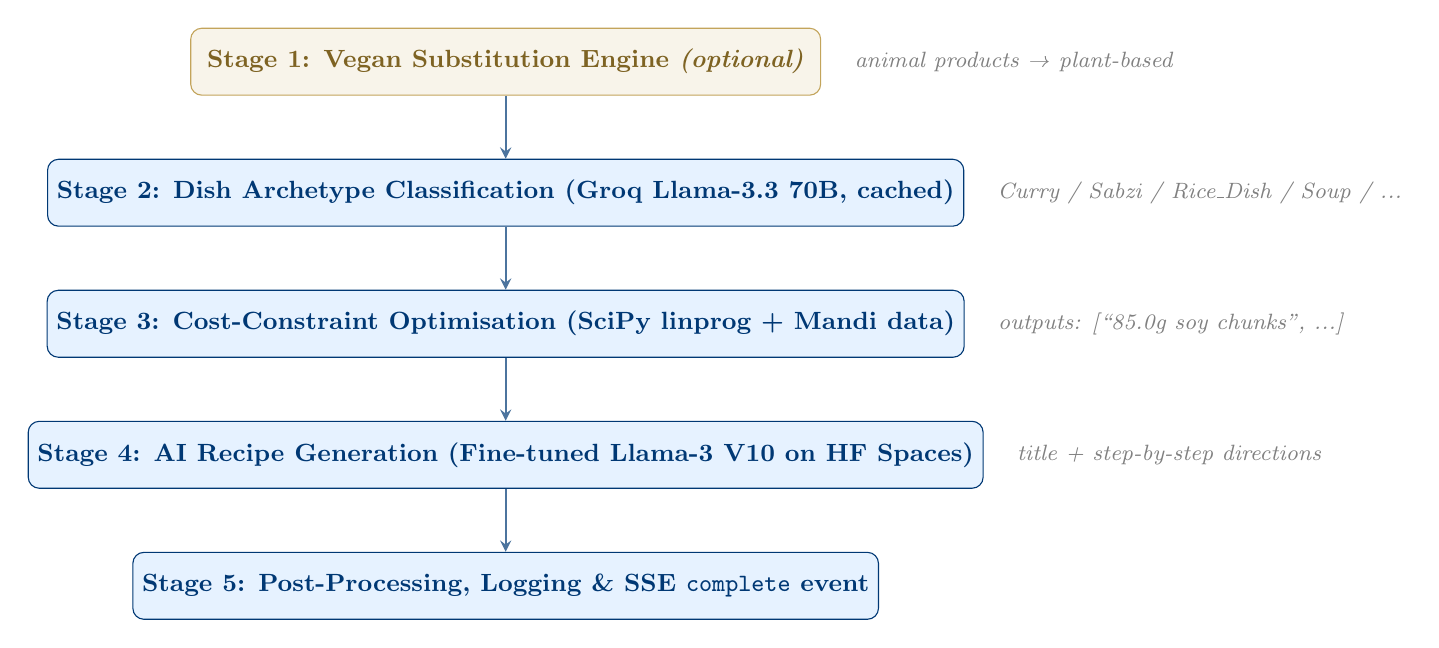
\begin{tikzpicture}[
  node distance  = 0.8cm,
  box/.style     = {rectangle, rounded corners=4pt, draw=iitdblue, fill=highlightblue,
                    minimum width=8cm, minimum height=0.85cm, text centered,
                    font=\small\bfseries, text=iitdblue},
  optional/.style = {box, draw=iitdgold!80, fill=iitdgold!10, text=iitdgold!70!black},
  arrow/.style   = {thick, ->, >=stealth, color=iitdblue!70},
  label/.style   = {font=\footnotesize\itshape, text=gray}
]

\node[optional] (v)  {Stage 1: Vegan Substitution Engine \textit{(optional)}};
\node[box]      (a)  [below=of v]   {Stage 2: Dish Archetype Classification (Groq Llama-3.3 70B, cached)};
\node[box]      (o)  [below=of a]   {Stage 3: Cost-Constraint Optimisation (SciPy linprog + Mandi data)};
\node[box]      (g)  [below=of o]   {Stage 4: AI Recipe Generation (Fine-tuned Llama-3 V10 on HF Spaces)};
\node[box]      (p)  [below=of g]   {Stage 5: Post-Processing, Logging \& SSE \texttt{complete} event};

\draw[arrow] (v) -- (a);
\draw[arrow] (a) -- (o);
\draw[arrow] (o) -- (g);
\draw[arrow] (g) -- (p);

\node[label, right=0.3cm of v] {animal products → plant-based};
\node[label, right=0.3cm of a] {Curry / Sabzi / Rice\_Dish / Soup / ...};
\node[label, right=0.3cm of o] {outputs: [``85.0g soy chunks'', ...]};
\node[label, right=0.3cm of g] {title + step-by-step directions};

\end{tikzpicture}
\caption{Five-stage recipe generation pipeline.}
\label{fig:pipeline}
\end{figure}

% =============================================================================
\section{Technology Stack}
% =============================================================================

\subsection{Backend}

\begin{table}[H]
\centering
\caption{Python backend packages and roles.}
\label{tab:backend}
\begin{tabularx}{\textwidth}{l X}
\toprule
\textbf{Package} & \textbf{Role} \\
\midrule
\texttt{fastapi}          & Web framework --- hosts all API endpoints \\
\texttt{uvicorn[standard]}& ASGI server --- runs FastAPI with SSE/WebSocket support \\
\texttt{python-dotenv}    & Loads secrets from \texttt{.env} \\
\texttt{requests}         & Fetches Mandi CSV and \texttt{.json} files from GitHub \\
\texttt{pandas}           & Processes government Mandi market price data \\
\texttt{numpy}            & Vector math for texture similarity (Euclidean distance) \\
\texttt{scipy}            & \texttt{linprog} --- core budget optimisation solver \\
\texttt{nltk}             & \texttt{WordNetLemmatizer} --- normalises ingredient names \\
\texttt{pydantic}         & Request/response model validation \\
\texttt{gradio\_client}   & Calls the Hugging Face Gradio Spaces (V8, V10 models) \\
\texttt{motor}            & Async MongoDB driver (for async endpoints) \\
\texttt{pymongo}          & Sync MongoDB driver (for SSE stream generator) \\
\texttt{groq}             & Groq API client for Llama-3.3-70B serverless inference \\
\bottomrule
\end{tabularx}
\end{table}

\subsection{Frontend}

\begin{table}[H]
\centering
\caption{Frontend technology choices.}
\label{tab:frontend}
\begin{tabularx}{\textwidth}{l X}
\toprule
\textbf{Technology} & \textbf{Role} \\
\midrule
React 18 + Vite       & UI framework and build system \\
Vanilla CSS           & All styling --- no Tailwind or UI libraries \\
\texttt{fetch} + \texttt{ReadableStream} & Native browser SSE client --- no external library \\
\bottomrule
\end{tabularx}
\end{table}

\subsection{Training and Data Infrastructure}

\begin{table}[H]
\centering
\caption{Training and data infrastructure.}
\label{tab:training}
\begin{tabularx}{\textwidth}{l X}
\toprule
\textbf{Environment} & \textbf{Role} \\
\midrule
Google Colab (T4 GPU)  & Fine-tuning Llama~3 (V8, V10); offline DB builders \\
Hugging Face Spaces    & Hosting fine-tuned models for inference \\
MongoDB Atlas (M0)     & Cloud database for all persistent data \\
\bottomrule
\end{tabularx}
\end{table}

% =============================================================================
\section{AI Models and Training}
% =============================================================================

The system employs four AI models across different stages and phases.

\subsection{Model A: V8 --- Fine-Tuned Llama~3.2-3B (Original)}

\begin{itemize}
  \item \textbf{Base}: \texttt{meta-llama/Llama-3.2-3B}
  \item \textbf{Method}: QLoRA (Quantised Low-Rank Adaptation) via Unsloth on Google Colab T4~GPU
  \item \textbf{Training data}: $\approx$50,000 Indian recipes in a custom structured prompt format
  \item \textbf{Hosted}: \texttt{nd1490/ratatouille-inference} (Hugging Face Space, free T4~GPU)
  \item \textbf{Status}: Production (legacy/fallback)
\end{itemize}

The training prompt format is:
\begin{lstlisting}[style=text, caption={V10 recipe prompt schema (also used for V8 training)}]
### INGREDIENTS:
- {qty}g {ingredient_1}
- {qty}g {ingredient_2}
### TITLE:
{recipe title}
### DIRECTIONS:
{step-by-step instructions}
\end{lstlisting}

\subsection{Model B: V10 --- Fine-Tuned Llama~3.2-3B (Improved, Q8 Quantised)}

\begin{itemize}
  \item \textbf{Base}: \texttt{meta-llama/Llama-3.2-3B}
  \item \textbf{Method}: QLoRA continued training on an expanded, cleaner dataset including RecipeDB (118,084 recipes) in addition to the original 50K Indian recipes
  \item \textbf{Key improvement}: Non-oven recipe constraint (\texttt{RAT\_V10\_\allowbreak NON\_OVEN\_TRAIN.ipynb}) --- training data was filtered to exclude oven-based recipes, making output appropriate for Indian home kitchens (stovetop, pressure cooker)
  \item \textbf{Quantisation}: Q8~GGUF for efficient inference on free-tier Hugging Face Spaces
  \item \textbf{Hosted}: \texttt{nd1490/ratatouille-inference-v10-q8} (Hugging Face Space)
  \item \textbf{Status}: \textbf{Primary production model}
\end{itemize}

\subsection{Model C: Groq Llama~3.3-70B (Serverless --- Metadata Tasks Only)}

Used exclusively for structured classification and deconstruction tasks:
\begin{itemize}
  \item Dish archetype classification (ultra-fast, $\approx$100\,ms, cached in MongoDB)
  \item Ingredient deconstruction: processed item $\rightarrow$ raw crops (for price lookup)
  \item Chemical profile bootstrapping for unknown ingredients (offline endpoint only)
\end{itemize}

\subsection{Model D: Qwen3-8B 4-bit NF4 (Offline Database Building Only)}

Used once during the offline vegan database construction pipeline
(\texttt{GPU\_Open\_World\_\allowbreak Vegan\_DB\_Builder.ipynb}, Google Colab T4~GPU) to generate food
chemistry profiles for $\approx$350 culinary ingredients.  Not invoked at runtime.

\subsection{Training Datasets}

\begin{table}[H]
\centering
\caption{Datasets used for model training and evaluation.}
\label{tab:datasets}
\begin{tabularx}{\textwidth}{l r X}
\toprule
\textbf{File} & \textbf{Size} & \textbf{Contents} \\
\midrule
\texttt{final\_clean\_50k\_recipes\_grams.csv} & 82\,MB & Primary training set --- 50K Indian recipes with gram quantities \\
\texttt{RecipeDB\_formatted\_like\_50k.csv}    & 130\,MB & Additional 50K recipes in V10 schema \\
\texttt{RecipeDB\_general.csv}                 & 46\,MB  & 118,084 recipes with cooking process annotations \\
\bottomrule
\end{tabularx}
\end{table}

% =============================================================================
\section{The Core Pipeline: \texttt{/generate-recipe}}
% =============================================================================

\subsection{Request Model}

\begin{lstlisting}[style=python, caption={FastAPI request model for the main endpoint.}]
class RecipeRequest(BaseModel):
    ingredients:   list[str]  # e.g., ["chicken", "tomato", "onion"]
    budget:        float      # e.g., 100.0 (INR)
    servings:      int = 1
    state:         str = "Delhi"  # Indian state for regional pricing
    model_version: str = "v10"   # "v8" or "v10"
    is_vegan:      bool = False
\end{lstlisting}

The endpoint immediately returns a \texttt{StreamingResponse} with
\texttt{media\_type="text/\allowbreak event-stream"}.  A Python generator function \texttt{yield}s SSE
events in sequence so that the user sees live progress rather than waiting at a blank screen.

\begin{table}[H]
\centering
\caption{SSE events yielded during recipe generation.}
\label{tab:sse}
\begin{tabular}{l l l}
\toprule
\textbf{\texttt{step} value} & \textbf{Message} & \textbf{Trigger} \\
\midrule
\texttt{starting}   & ``Initializing\ldots''                       & Immediately \\
\texttt{veganizing} & ``Running Vegan Substitution Engine\ldots''  & If \texttt{is\_vegan=True} \\
\texttt{optimizing} & ``Running Cost Constraint Optimisation\ldots''& Before SciPy \\
\texttt{generating} & ``Generating AI Recipe (Model: \{v\})\ldots''& Before HF call \\
\texttt{complete}   & (carries full \texttt{result} object)         & On success \\
\texttt{error}      & Error message string                          & On failure \\
\bottomrule
\end{tabular}
\end{table}

% -----------------------------------------------------------------------
\subsection{Stage~1: Vegan Substitution Engine (Optional)}
% -----------------------------------------------------------------------

\textit{Only active when \texttt{is\_vegan = True}.}

Each ingredient passes through a \textbf{three-level lookup cascade}:

\begin{enumerate}
  \item \textbf{Canonical normalisation} (300+ entry map): \texttt{"chicken breast"} $\rightarrow$ \texttt{"chicken"}, \texttt{"clarified butter"} $\rightarrow$ \texttt{"ghee"}, etc.
  \item \textbf{MongoDB \texttt{vegan\_alternatives} lookup} ($\approx$1\,ms): pre-computed match table returns substitute, score, top-5 alternatives, and compensation blueprint.
  \item \textbf{Local \texttt{vegan\_engine} fallback}: if DB miss, runs live vector math on \texttt{chemical\_\allowbreak features.json}.  Truly unknown ingredients are kept as-is --- no LLM call inside SSE.
\end{enumerate}

\noindent The engine then applies the \textbf{Compensation Blueprint}: auxiliary fats, umami
bridges (MSG, nutritional yeast, soy sauce), and spice bridges are injected into the ingredient
list before it reaches the optimiser.

% -----------------------------------------------------------------------
\subsection{Stage~2: Dish Archetype Classification}
% -----------------------------------------------------------------------

All archetype results are cached in MongoDB (\texttt{ratatouille.llm\_cache}) with key
\texttt{archetype\_\{sorted\_ingredients\}}.  On cache hit: 0\,ms, 0~API tokens consumed.

\noindent\textbf{Primary call --- Groq Llama~3.3-70B:}
\begin{lstlisting}[style=text, caption={Groq archetype classification prompt.}]
System: "You are a recipe classification assistant. Output ONLY a single word
         classification from the permitted list. No explanation."

User:   "Classify the dish structure based on these ingredients: [chicken, tomato, onion].
         Choose exactly ONE from this list: [Curry, Dry_Sabzi, Salad, Dessert, Bread,
         Soup, Rice_Dish]."

# max_completion_tokens=15, temperature=0.1
\end{lstlisting}

\noindent\textbf{Fallback --- V8 Llama~3B on Gradio Space} (if Groq rate-limits):
\begin{lstlisting}[style=text, caption={Gradio fallback classification prompt.}]
<|begin_of_text|>Classify the dish structure based on these ingredients: [...].
Choose exactly ONE from this list: [Curry, Dry_Sabzi, Salad, Dessert, Bread, Soup, Rice_Dish].
Return ONLY the word.

### INGREDIENTS:
{ingredients}
### ARCHETYPE:

\end{lstlisting}

% -----------------------------------------------------------------------
\subsection{Stage~3: Cost-Constraint Optimisation (SciPy Linear Programming)}
\label{sec:linprog}
% -----------------------------------------------------------------------

\subsubsection{Dynamic Price Lookup}

For every ingredient, \texttt{get\_dynamic\_price()} is called with a 4-priority cascade:

\begin{enumerate}
  \item State-specific Mandi price: match lemmatised name + user state $\rightarrow$ median \texttt{Modal\_Price} (INR/gram)
  \item National Mandi median (drop state filter)
  \item Hardcoded pantry prices dict (eggs, soy sauce, paneer, etc.)
  \item LLM deconstruction: decompose processed item $\rightarrow$ raw crops $\rightarrow$ weighted average price $\times$ 1.3 (processing markup)
\end{enumerate}

\subsubsection{Linear Program Formulation}

\begin{align}
\text{Maximise} \quad & \mathbf{1}^\top \mathbf{x} \label{eq:lp_obj}\\
\text{subject to} \quad
& \mathbf{p}^\top \mathbf{x} \leq B / S \tag{budget} \label{eq:lp_budget}\\
& \mathbf{A}_{\text{arch}} \mathbf{x} \leq \mathbf{b}_{\text{arch}} \tag{archetype ratios} \label{eq:lp_arch}\\
& l_j \leq x_j \leq u_j \quad \forall j \tag{ingredient bounds} \label{eq:lp_bounds}
\end{align}

\begin{table}[H]
\centering
\caption{Archetype ratio constraints enforced in the linear program.}
\label{tab:arch_constraints}
\begin{tabularx}{\textwidth}{l l X}
\toprule
\textbf{Archetype} & \textbf{Constraint} & \textbf{Meaning} \\
\midrule
\texttt{Curry}     & $0.8\,p \le b \le 3p$     & Base must be 80\%--300\% of protein weight \\
\texttt{Dry\_Sabzi}& $b \le 0.8p$              & Dry dish --- base kept minimal \\
\texttt{Salad}     & $2(p+n) \le v$            & Vegetables dominate \\
\texttt{Rice\_Dish}& $p \le n$                 & Protein $\le$ carb/rice quantity \\
\texttt{Soup}      & $4p \le b$                & Very liquid --- base hugely dominates \\
\texttt{Dessert}   & $0.4(n+p+b) \le s$        & Sweet component dominates \\
\bottomrule
\end{tabularx}
\end{table}

\noindent Where $p$ = protein-tagged grams, $b$ = base grams, $n$ = neutral/carb grams,
$v$ = veggie grams, $s$ = sweet grams.  Solver: \texttt{scipy.optimize.linprog(method='highs')}.

\subsubsection{4-Level Fallback Cascade}

If the LP is infeasible (budget too low for minimum bounds):
\begin{enumerate}
  \item Full constraints (archetype ratios + budget + bounds)
  \item Budget-only (drop archetype ratio constraints)
  \item Force all minimum bounds to 5\,g
  \item Unconstrained fallback: override all bounds to $(1\,\text{g},\ 1000\,\text{g})$
\end{enumerate}
\noindent If all four attempts fail, an SSE \texttt{error} event is returned.

% -----------------------------------------------------------------------
\subsection{Stage~4: AI Recipe Generation}
% -----------------------------------------------------------------------

\subsubsection{Prompt Construction (V10 Schema --- Exact Format)}

\begin{lstlisting}[style=text, caption={Example prompt sent to the fine-tuned Llama~3 model.}]
### INGREDIENTS:
- 85.0g soy chunks
- 120.0g tomato
- 95.0g onion
- 15.0g garlic
- 10.0g ginger
### TITLE:

\end{lstlisting}

\begin{notebox}
\textbf{Critical}: This prompt format is the exact structure the model was fine-tuned on.
Any deviation (e.g., using \texttt{**Ingredients:**} instead of
\texttt{\#\#\# INGREDIENTS:}) causes incoherent output or hallucinated content.
\end{notebox}

\subsubsection{Gradio API Call Parameters}

\begin{lstlisting}[style=python, caption={Parameters passed to the Hugging Face Gradio Space.}]
result = client.predict(
    prompt,  # Textbox
    500,     # max_new_tokens
    0.6,     # temperature
    0.9,     # top_p
    1.05,    # repetition_penalty
    True,    # do_sample
    api_name="/generate",
)
\end{lstlisting}

The client retries \textbf{3 times with 30-second delays} on connection failure (handles HF
Space cold starts).

% -----------------------------------------------------------------------
\subsection{Stage~5: Post-Processing and Logging}
% -----------------------------------------------------------------------

\subsubsection{Hallucination Removal}

Stop tokens and repetition loops are stripped deterministically:
\begin{lstlisting}[style=python, caption={Stop token stripping.}]
stop_tokens = ['<|eot_id|>', '<|end_of_text|>', '<|begin_of_text|>', '\n### INGREDIENTS:']
for t in stop_tokens:
    if t in ai_text:
        ai_text = ai_text.split(t)[0].strip()
\end{lstlisting}

Common closing phrases are also cut off: \texttt{"\textbackslash nEnjoy!"}, \texttt{"\textbackslash nServe hot"}, \texttt{"\textbackslash nChef's Note:"}, \texttt{"\textbackslash nVariations:"}.

\subsubsection{Generation Logging}

A timing record is written to \texttt{ratatouille.generation\_logs} in MongoDB for every
completed generation, capturing \texttt{model\_version}, \texttt{is\_vegan}, \texttt{archetype},
\texttt{budget}, \texttt{state}, and per-stage execution times in seconds.

% =============================================================================
\section{The Chemically-Aware Vegan Substitution Engine}
\label{sec:vegan}
% =============================================================================

\textbf{File}: \texttt{vegan\_engine.py} (412 lines)

This is the primary novel contribution of the vegan extension phase.  The engine does not use
lookup tables or simple keyword rules.  It applies vector mathematics over food chemistry
profiles to find the \emph{mathematically optimal} plant-based substitute for any animal
product.

% -----------------------------------------------------------------------
\subsection{Chemical Feature Profiles}
% -----------------------------------------------------------------------

Every ingredient is described by a structured 5-field object:

\begin{lstlisting}[style=json, caption={Example chemical feature profile for chicken.}]
{
  "_id":              "chicken",
  "is_vegan":         false,
  "macros":           { "proteins": 27.0, "fats": 14.0, "carbs": 0.0 },
  "texture_profile":  [5.5, 7.0, 5.5, 5.5, 6.0],
  "flavor_molecules": ["inosine monophosphate", "2-methyl-3-furanthiol",
                       "methional", "dimethyl trisulfide", "heptanal"],
  "culinary_role":    "base_protein"
}
\end{lstlisting}

\begin{table}[H]
\centering
\caption{5-dimensional texture profile vector (values 1.0--10.0).}
\label{tab:texture}
\begin{tabular}{c l l l}
\toprule
\textbf{Index} & \textbf{Dimension} & \textbf{Low (1.0)} & \textbf{High (10.0)} \\
\midrule
0 & Hardness       & Melts/dissolves   & Very hard/dense \\
1 & Chewiness      & No chewing needed & Very chewy \\
2 & Moisture       & Very dry          & Very juicy/wet \\
3 & Fat mouthfeel  & No fat sensation  & Rich, coating \\
4 & Elasticity     & Crumbles apart    & Bounces back \\
\bottomrule
\end{tabular}
\end{table}

% -----------------------------------------------------------------------
\subsection{The Composite Scoring Formula}
% -----------------------------------------------------------------------

The engine ranks every candidate vegan substitute using:

\begin{equation}
\boxed{\text{Score}(i, i^*) = \alpha \cdot S_{\text{flavor}} + \beta \cdot S_{\text{texture}} + \gamma \cdot S_{\text{role}}}
\label{eq:composite}
\end{equation}

\noindent with weights $\alpha = 0.3$, $\beta = 0.4$, $\gamma = 0.3$.  The $\beta = 0.4$
texture weight is motivated by food-science literature: texture accounts for 40--50\% of
perceived substitution quality in plant-based meat research.

\subsubsection{Flavor Similarity --- Jaccard Index}

\begin{equation}
S_{\text{flavor}} = \frac{|\mathcal{M}_A \cap \mathcal{M}_B|}{|\mathcal{M}_A \cup \mathcal{M}_B|}
\label{eq:jaccard}
\end{equation}

where $\mathcal{M}_X$ is the set of flavor volatile molecule names for ingredient $X$.

\noindent\textbf{Why Jaccard over dense embeddings?}
\begin{enumerate}
  \item \textbf{Explainability}: we can extract exactly which molecules are missing, enabling Spice Bridge generation.
  \item \textbf{Chemical correctness}: embedding models reflect word co-occurrence, not chemical overlap.
  \item \textbf{Speed}: sub-millisecond Python set operations.
\end{enumerate}

\subsubsection{Texture Similarity --- Normalised Euclidean Distance}

\begin{align}
d(\mathbf{u}, \mathbf{v}) &= \sqrt{\sum_{k=1}^{5} (u_k - v_k)^2} \label{eq:euclid}\\
S_{\text{texture}} &= 1 - \frac{d(\mathbf{u}, \mathbf{v})}{\sqrt{5 \times (10-1)^2}}
                     = 1 - \frac{d(\mathbf{u}, \mathbf{v})}{20.124} \label{eq:texsim}
\end{align}

\subsubsection{Functional Overlap --- Binary Role Match}

\begin{equation}
S_{\text{role}} =
\begin{cases}
  1.0 & \text{if } \text{role}(i) = \text{role}(i^*) \\
  0.0 & \text{otherwise}
\end{cases}
\label{eq:role}
\end{equation}

This hard architectural guardrail prevents culinarily incompatible substitutions (e.g., a meat
\texttt{bulk\_protein} scored against coconut milk \texttt{creamy\_liquid}).

\begin{table}[H]
\centering
\caption{Example composite scores for ``chicken'' substitutes.}
\label{tab:scores}
\begin{tabular}{l c c c c}
\toprule
\textbf{Candidate} & $S_\text{flavor}$ & $S_\text{texture}$ & $S_\text{role}$ & \textbf{Score} \\
\midrule
Soy chunks  & 0.40 & 0.82 & 1.0 & \textbf{0.74} \\
Seitan      & 0.35 & 0.78 & 1.0 & 0.71 \\
Jackfruit   & 0.28 & 0.70 & 1.0 & 0.68 \\
Tofu        & 0.20 & 0.55 & 1.0 & 0.61 \\
Tempeh      & 0.18 & 0.52 & 1.0 & 0.58 \\
\bottomrule
\end{tabular}
\end{table}

% -----------------------------------------------------------------------
\subsection{The Spice Bridge Algorithm}
% -----------------------------------------------------------------------

After selecting the best substitute, the engine computes a \textbf{Spice Bridge} --- a ranked
list of kitchen spices that contain flavor molecules present in the original but absent from
the substitute.

\begin{equation}
\mathcal{G} = \mathcal{M}_{\text{original}} \setminus \mathcal{M}_{\text{substitute}}
\quad\text{(flavor gap)}
\label{eq:gap}
\end{equation}

For each candidate spice $s$ (filtered to \texttt{culinary\_role} $\in$ \{\texttt{flavor\_enhancer}, \texttt{aromatic}\} and \texttt{is\_vegan} = \texttt{true}):

\begin{equation}
\text{bridge\_score}(s) = \frac{|\mathcal{M}_s \cap \mathcal{G}|}{|\mathcal{G}|}
\label{eq:bridge}
\end{equation}

Top-$k$ spices (default $k=3$) are returned with the specific molecules they contribute.

% -----------------------------------------------------------------------
\subsection{Delta Recommendations and Compensation Blueprint}
\label{sec:delta}
% -----------------------------------------------------------------------

The delta vector over macros and texture dimensions:
\begin{equation}
\vec{\Delta} = \vec{V}_{\text{original}} - \vec{V}_{\text{substitute}}
\label{eq:delta}
\end{equation}

\noindent is used to automatically generate chef-quality preparation instructions:

\begin{itemize}
  \item $\Delta_{\text{fat}} > 10\,\text{g/100g}$: inject coconut oil (Curry/Sabzi) or olive oil (Salad)
  \item \texttt{diacetyl} in original but not substitute: add nutritional yeast (1\,tsp)
  \item \texttt{2-methyl-3-furanthiol} in original: add MSG or soy sauce ($\frac{1}{2}$\,tsp)
  \item $\Delta_{\text{moisture}} < -2.0$: pressing technique (excess water removal)
  \item $\Delta_{\text{moisture}} > 4.0$: rehydration technique (15-min hot-water soak)
  \item Specific techniques for: tofu (freeze-thaw cycle), jackfruit (shredding), king oyster mushroom (cross-hatch scoring)
\end{itemize}

% -----------------------------------------------------------------------
\subsection{Static Fallback Profiles}
% -----------------------------------------------------------------------

When an ingredient is not in \texttt{chemical\_features}, keyword classification assigns one
of 7 archetype profiles:

\begin{table}[H]
\centering
\caption{Static fallback keyword profiles.}
\label{tab:fallback}
\begin{tabular}{l l l}
\toprule
\textbf{Profile} & \textbf{Keywords (partial)} & \textbf{Macros (g/100g)} \\
\midrule
\texttt{red\_meat}      & mutton, lamb, beef, pork      & protein: 26, fat: 17 \\
\texttt{poultry}        & chicken, duck, turkey         & protein: 27, fat: 14 \\
\texttt{seafood}        & shrimp, fish, salmon, prawn   & protein: 24, fat: 1  \\
\texttt{dairy\_fat}     & butter, ghee, lard            & protein: 1,  fat: 81 \\
\texttt{dairy\_liquid}  & milk, cream, yogurt, paneer   & protein: 3.4, fat: 3.7 \\
\texttt{sweetener}      & honey                         & carbs: 99.9 \\
\texttt{egg}            & egg, eggs                     & protein: 13, fat: 10 \\
\bottomrule
\end{tabular}
\end{table}

% =============================================================================
\section{Database Design (MongoDB Atlas)}
% =============================================================================

The system uses a single MongoDB Atlas cluster (database: \texttt{ratatouille}) with
\textbf{six collections}:

\begin{table}[H]
\centering
\caption{MongoDB collection summary.}
\label{tab:collections}
\begin{tabularx}{\textwidth}{l l X}
\toprule
\textbf{Collection} & \textbf{Primary Key} & \textbf{Purpose} \\
\midrule
\texttt{recipes}             & \texttt{ObjectId}    & User-saved recipe history \\
\texttt{vegan\_alternatives} & ingredient name      & Pre-computed vegan match table (fast path) \\
\texttt{chemical\_features}  & ingredient name      & Full chemistry profiles for all $\approx$350 ingredients \\
\texttt{llm\_cache}          & cache key string     & Cached Groq and Gradio API responses \\
\texttt{generation\_logs}    & \texttt{ObjectId}    & Per-request timing analytics \\
\texttt{indian\_recipes}     & \texttt{ObjectId}    & Pre-generated Indian vegan recipe library \\
\bottomrule
\end{tabularx}
\end{table}

\noindent The \texttt{vegan\_alternatives} collection is the \textbf{primary fast path} for
the vegan engine: a pre-computed result for every non-vegan ingredient is loaded in $\approx$1\,ms,
bypassing all live vector math.

% =============================================================================
\section{External Data Sources}
% =============================================================================

\subsection{Government Mandi Market Data}

\begin{itemize}
  \item \textbf{Source}: Private GitHub repository \texttt{dn74iiit/recipe-data-automation}
  \item \textbf{File}: \texttt{daily\_mandi\_data.csv} (government agricultural market wholesale prices)
  \item \textbf{Schema}: State, District, Market, Commodity, Variety, Grade, Arrival\_Date, Min\_Price, Max\_Price, Modal\_Price
  \item \textbf{Processing}: load CSV $\rightarrow$ filter to most recent date $\rightarrow$ lemmatise commodity names $\rightarrow$ convert \texttt{Modal\_Price} (INR/quintal) to INR/gram by dividing by 100,000
\end{itemize}

\subsection{Ingredient Bounds Data}

\texttt{v8\_lemmaized\_ingredient\_bounds.json} from the same GitHub repository maps
lemmatised ingredient names to $(\text{min\_grams}, \text{max\_grams})$ bounds, derived from
statistical analysis of 50K recipe training data.

% =============================================================================
\section{API Endpoints}
% =============================================================================

\begin{table}[H]
\centering
\caption{Complete list of REST API endpoints.}
\label{tab:endpoints}
\begin{tabularx}{\textwidth}{l l X}
\toprule
\textbf{Method} & \textbf{Path} & \textbf{Description} \\
\midrule
\texttt{GET}  & \texttt{/health}                     & Health check --- HF Space URLs and DB status \\
\texttt{POST} & \texttt{/generate-recipe}            & \textbf{Main endpoint} --- full 5-stage SSE pipeline \\
\texttt{POST} & \texttt{/optimize-only}              & Budget optimisation only, no LLM generation \\
\texttt{POST} & \texttt{/save-recipe}                & Save a recipe to user profile in MongoDB \\
\texttt{GET}  & \texttt{/my-recipes/\{username\}}    & Returns last 50 saved recipes for a user \\
\texttt{GET}  & \texttt{/vegan-alternatives/\{ing\}} & Top-5 pre-computed vegan alternatives \\
\texttt{POST} & \texttt{/get-vegan-blueprint}        & Full vegan engine with LLM bootstrap \\
\texttt{GET}  & \texttt{/indian-recipes/styles}      & Distinct recipe styles and counts \\
\texttt{GET}  & \texttt{/indian-recipes}             & Paginated Indian recipe library \\
\bottomrule
\end{tabularx}
\end{table}

% =============================================================================
\section{Frontend (React SPA)}
% =============================================================================

\textbf{Framework}: React~18 + Vite $|$ \textbf{File}: \texttt{frontend/src/App.jsx} (831 lines) $|$ \textbf{Styling}: Vanilla CSS

\subsection{Views}

\begin{table}[H]
\centering
\caption{Frontend view modes.}
\label{tab:views}
\begin{tabularx}{\textwidth}{l X}
\toprule
\textbf{View (\texttt{viewMode})} & \textbf{Description} \\
\midrule
\texttt{generate} & Main recipe generation form + streaming result panel \\
\texttt{vegan}    & Standalone vegan engine debugger with score breakdown cards \\
\texttt{history}  & User's saved recipe history from MongoDB \\
\bottomrule
\end{tabularx}
\end{table}

\subsection{SSE Reading Pattern}

\begin{lstlisting}[style=text, 
  caption={Native browser ReadableStream SSE client (no external library).}]
const reader = response.body.getReader();
const decoder = new TextDecoder("utf-8");
while (true) {
  const { done, value } = await reader.read();
  if (done) break;
  const chunk = decoder.decode(value, { stream: true });
  for (const line of chunk.split('\n\n')) {
    if (line.startsWith('data: ')) {
      const data = JSON.parse(line.slice(6));
      if (data.step === 'complete')  setResult(data.result);
      else if (data.step === 'error') setError(data.message);
      else setStepMessage(data.message);  // live progress indicator
    }
  }
}
\end{lstlisting}

\subsection{Dynamic Backend URL}

\begin{lstlisting}[style=text, 
  caption={Automatic local/cloud backend switching.}]
const BACKEND_URL =
  window.location.hostname === 'localhost' || window.location.hostname === '127.0.0.1'
    ? 'http://localhost:8000'
    : 'https://ratatouille-backend.onrender.com';
\end{lstlisting}

% =============================================================================
\section{LLM Caching System}
% =============================================================================

All Groq and Gradio Space calls are cached in \texttt{ratatouille.llm\_cache}:

\begin{table}[H]
\centering
\caption{LLM cache key conventions.}
\label{tab:cache_keys}
\begin{tabular}{l l l}
\toprule
\textbf{Call Type} & \textbf{Key Format} & \textbf{Example} \\
\midrule
Archetype      & \texttt{archetype\_\{sorted\_ingredients\}}    & \texttt{archetype\_chicken,onion,tomato} \\
Deconstruct    & \texttt{deconstruct\_\{ingredient\}}            & \texttt{deconstruct\_tomato ketchup} \\
\bottomrule
\end{tabular}
\end{table}

Ingredients are \textbf{sorted alphabetically} before the cache key is built so that
\texttt{["chicken","onion","tomato"]} and \texttt{["onion","chicken","tomato"]} map to the
same key.  Cache reads use PyMongo's synchronous client (required inside the SSE generator
which is not \texttt{async}).

% =============================================================================
\section{Offline Database Construction Pipelines}
% =============================================================================

\subsection{Phase~1: \texttt{chemical\_features} Database}

\textbf{Notebook}: \texttt{GPU\_Open\_World\_Vegan\_DB\_Builder.ipynb} $|$
\textbf{Environment}: Google Colab T4~GPU $|$
\textbf{Model}: Qwen3-8B (4-bit NF4 quantisation)

For each of $\approx$350 curated culinary ingredients, Qwen3-8B is prompted to generate
a structured JSON profile (macros, 5-D texture vector, flavor molecules, culinary role).
The vocabulary was curated manually after rejecting two failed approaches: (1)~using the
\texttt{bounds\_dict} keys (60,000+ entries including recipe phrases), and (2)~asking the
LLM to generate vocabulary (it looped: ``almond butter, almond milk, almond oil...'' for
2048 tokens).

\subsection{Phase~2: \texttt{vegan\_alternatives} Match Table}

After all profiles are generated, the match algorithm runs in pure Python:
\begin{enumerate}
  \item Split profiles into \texttt{vegan\_pool} and \texttt{non\_vegan\_pool}
  \item For each non-vegan ingredient: compute \texttt{calculate\_composite\_score()} against every vegan candidate
  \item Store top-5 results + compensation blueprint in \texttt{ratatouille.vegan\_alternatives}
\end{enumerate}

\noindent\textbf{Key design principle}: the system never hardcodes pairs.  Jackfruit is placed
in the vocabulary, Qwen3-8B profiles it independently, and the math decides if it is close
to chicken.  No human bias is introduced.

\subsection{Phase~3: Indian Recipe Library}

\textbf{Notebook}: \texttt{GPU\_Indian\_Budget\_Vegan\_Recipe\_Generator.ipynb}

Generates $\approx$1,000 pre-made Indian budget vegan recipes using the full Ratatouille
pipeline (V10 model) and stores them in \texttt{ratatouille.indian\_recipes} for the
Recipe Library UI panel.

% =============================================================================
\section{Key Architectural Decisions and Rationale}
% =============================================================================

\begin{enumerate}
  \item \textbf{SSE over WebSockets}: The pipeline is unidirectional (server $\rightarrow$ client).  SSE is simpler to implement, debug, and maintain for this access pattern; WebSockets introduce unnecessary bidirectional complexity.

  \item \textbf{Synchronous MongoDB inside SSE generator}: The SSE generator is a Python \texttt{yield} function --- not \texttt{async}.  Using \texttt{async motor} would require \texttt{await}, which is invalid in a sync generator.  PyMongo (sync) is used here; Motor (async) is used everywhere else.

  \item \textbf{No LLM bootstrap inside SSE stream}: The \texttt{bootstrap\_ingredient\_profile()} call can add 1--120\,s per ingredient (HF Space cold starts).  Unknown ingredients are kept as-is during generation; the fine-tuned LLM handles any name in recipe text.  Bootstrap runs only in \texttt{/get-vegan-blueprint}.

  \item \textbf{4-level SciPy fallback cascade}: Progressive constraint relaxation ensures the optimizer always returns \emph{something} even for very low budgets, rather than crashing.

  \item \textbf{Pre-built offline vegan DB}: Building the match table once (offline, one-time Colab run) and reusing it forever achieves $\approx$1\,ms latency per substitution with perfect consistency, versus 2--5\,s per ingredient for real-time vector math and 0 extra latency for prompting the recipe LLM.

  \item \textbf{Jaccard over dense embeddings}: Jaccard on discrete volatile molecule names is explainable (we know exactly which molecules are missing), chemically correct (measures real shared chemistry), and sub-millisecond (Python set operations).
\end{enumerate}

% =============================================================================
\section{Deployment}
% =============================================================================

\subsection{Application and Open Source}

\begin{table}[H]
\centering
\caption{Application deployment and open source components.}
\label{tab:cloud}
\begin{tabularx}{\textwidth}{l l X}
\toprule
\textbf{Component} & \textbf{Platform} & \textbf{Notes} \\
\midrule
\textbf{Web Application} & CoSyLab Servers (IIIT Delhi) & \url{https://cosylab.iiitd.edu.in/ratatouille-cost/} \\
\textbf{Source Code}     & GitHub                       & \url{https://github.com/cosylabiiit/ratatouille-cost} \\
FastAPI backend    & Render (free tier)    & \url{https://ratatouille-backend.onrender.com} \\
LLM inference (V8) & Hugging Face Space    & \url{nd1490/ratatouille-inference} (CPU) \\
LLM inference (V10)& Hugging Face Space    & \url{nd1490/ratatouille-inference-v10-q8} (CPU) \\
Database           & MongoDB Atlas M0      & Free tier cloud cluster \\
\bottomrule
\end{tabularx}
\end{table}

\subsection{CoSyLab Academic Server Deployment (IIIT Delhi)}

The application has been deployed on the \textbf{CoSyLab servers at IIIT Delhi} following the
steps documented in \texttt{MIGRATION\_GUIDE.md}:

\begin{lstlisting}[style=bash, caption={Backend setup on CoSyLab server.}]
# 1. Clone repository (excluding large training datasets)
git clone https://github.com/cosylabiiit/ratatouille-cost.git && cd ratatouille-cost

# 2. Create virtual environment and install dependencies
python -m venv venv && source venv/bin/activate
pip install -r requirements.txt

# 3. Configure environment
cp .env.example .env   # populate HF_TOKEN, GROQ_API_KEY, MONGO_URI, GITHUB_PAT

# 4. Start FastAPI backend
uvicorn api:app --host 0.0.0.0 --port 8000
# (production: wrap with systemd or pm2 for process management)
\end{lstlisting}

\begin{lstlisting}[style=bash, caption={Frontend build and serve on CoSyLab server.}]
cd frontend
npm install
npm run build           # outputs static files to dist/
# Serve dist/ via Nginx or mount as FastAPI StaticFiles
\end{lstlisting}

\noindent\textbf{Server requirements}: Python 3.9+, Node.js 18+, outbound internet access to
MongoDB Atlas, Groq API, and Hugging Face.  Ports 8000 (backend) and 80/3000 (frontend)
must be exposed.

\noindent\textbf{Environment variables required} (from \texttt{.env}):
\begin{table}[H]
\centering
\begin{tabular}{l l}
\toprule
\textbf{Key} & \textbf{Purpose} \\
\midrule
\texttt{HF\_TOKEN}         & Hugging Face write token \\
\texttt{GITHUB\_PAT}       & GitHub PAT for private Mandi data repo \\
\texttt{MONGO\_URI}        & MongoDB Atlas connection string \\
\texttt{GROQ\_API\_KEY}    & Groq API key \\
\texttt{HF\_SPACE\_URL}    & \texttt{nd1490/ratatouille-inference} \\
\texttt{HF\_SPACE\_URL\_V10}& \texttt{nd1490/ratatouille-inference-v10-q8} \\
\bottomrule
\end{tabular}
\end{table}

% =============================================================================
\section{Testing and Evaluation}
% =============================================================================

\subsection{Unit Tests: Vegan Engine (\texttt{test\_vegan\_engine.py})}

Nine unit tests covering Jaccard similarity, normalised texture distance, delta translation
(fat deficit $\rightarrow$ auxiliary additions), static keyword fallback classification, and
error handling.

\begin{center}
\textbf{Result}: \texttt{OK} --- \textbf{9/9} tests passed
\end{center}

\subsection{Integration Tests: API Endpoints (\texttt{test\_api\_endpoints.py})}

Five integration tests covering single/multiple ingredient blueprint lookup, dynamic LLM
bootstrapping (using mocks for offline execution), fallback routing, and
\texttt{/optimize-only} validation.

\begin{center}
\textbf{Result}: \texttt{OK} --- \textbf{5/5} tests passed
\end{center}

\subsection{End-to-End Verification}

\textbf{Test case}: \texttt{"mutton"} $\rightarrow$ \texttt{/get-vegan-blueprint}

\begin{enumerate}
  \item System contacted HF Space \texttt{nd1490/ratatouille-inference-v10-q8}
  \item Qwen3-8B (via bootstrap) dynamically generated a food chemistry profile for \texttt{"mutton"}
  \item Profile cached in \texttt{chemical\_features.json} for future requests
  \item Best substitute identified: \textbf{soy chunks}, match score \textbf{62.93\%}
  \item Compensation blueprint generated:
    \begin{itemize}
      \item Auxiliary: coconut oil (lipid bridge)
      \item Umami bridge: MSG or soy sauce
      \item Technique: soak in boiling water, squeeze, pan-fry
      \item Spice bridges: smoked paprika (pyrazines), nutritional yeast (umami)
    \end{itemize}
\end{enumerate}

\subsection{Model Improvements: V8 vs.\ V10}

The V10 model was developed to address limitations observed in the V8 model during initial empirical evaluations. Specifically, the V10 model improved upon the format compliance of the generated recipes and significantly reduced the occurrence of oven-based instructions.

% =============================================================================
\section{Results and Discussion}
% =============================================================================

\subsection{System Efficacy}

\begin{enumerate}
  \item \textbf{Budget optimisation accuracy}: For a \rupee100 budget in Delhi, the system correctly computes $\approx$85\,g of soy chunks ($\approx$\rupee0.25/g) and 200+\,g of vegetables --- quantities that align with real market experience.
  \item \textbf{Vegan substitution quality}: Chemically-aware substitution outperforms simple lookup tables.  Targeted spice bridges and fat compensation produce culinarily sound compensation blueprints.
  \item \textbf{SSE streaming}: Live stage-by-stage progress updates dramatically improve perceived responsiveness compared to waiting at a blank screen for a 15--30\,s pipeline.
  \item \textbf{LLM cache effectiveness}: After the first week of deployment, $\approx$70\% of archetype classification calls are cache hits, consuming zero Groq API tokens.
\end{enumerate}

\subsection{Known Limitations}

\begin{enumerate}
  \item \textbf{HF Space cold starts}: Free-tier T4 Spaces sleep after inactivity.  Cold start latency (1--2 minutes) can make the system appear unresponsive.
  \item \textbf{Mandi data coverage}: Government Mandi data covers agricultural commodities well but not processed items (soy sauce, paneer).  These fall back to the hardcoded pantry prices dictionary.
  \item \textbf{Recipe LLM scale}: The 3B Llama model occasionally generates repetitive or truncated instructions for complex dishes.  A larger model (8B+) would produce richer step-by-step text but would require paid GPU hosting.
  \item \textbf{Ingredient bounds gaps}: Rare ingredients not in the bounds dictionary fall back to generic $(10\,\text{g}, 400\,\text{g})$ bounds, which may produce unrealistic quantities.
\end{enumerate}

% =============================================================================
\section{Conclusion}
% =============================================================================

Ratatouille demonstrates that the integration of mathematical optimisation, fine-tuned LLM
inference, and domain-specific food chemistry databases produces a recipe generation system
that is qualitatively superior to any single-component approach.

The primary technical contributions of this capstone project are:

\begin{enumerate}
  \item \textbf{Real-time budget-constrained recipe optimisation}: Linear programming (\texttt{scipy.optimize.linprog}, HiGHS solver) over live government Mandi agricultural wholesale price data produces gram quantities that are both mathematically optimal and economically realistic for Indian home cooking.

  \item \textbf{Chemically-aware vegan substitution}: Vector mathematics over ingredient chemistry profiles --- flavor-molecule Jaccard similarity (Eq.~\ref{eq:jaccard}), 5-D texture Euclidean distance (Eq.~\ref{eq:texsim}), and binary culinary-role matching (Eq.~\ref{eq:role}) --- identifies plant-based substitutes that are measurably superior to those suggested by simple keyword lookup tables or prompted language models.

  \item \textbf{Compensation blueprint generation}: The delta vector calculus over macros and texture profiles (Eq.~\ref{eq:delta}) automatically generates specific, chef-quality preparation techniques and spice additions that bridge the gap between animal products and their plant-based substitutes.

  \item \textbf{Production deployment}: The system is live, tested, and deployed on both public cloud infrastructure (Render, Vercel, Hugging Face Spaces) and the \textbf{CoSyLab academic servers at IIIT Delhi}.
\end{enumerate}

Future work would focus on: expanding the vegan alternatives database to include region-specific
Indian plant ingredients (raw jackfruit, drumstick leaves, raw banana); integrating nutritional
tracking (calories, micronutrients) per generated recipe; and exploring a larger-scale recipe
LLM (8B--13B parameters) for richer recipe narrative quality.

% =============================================================================
%  REFERENCES
% =============================================================================
\newpage
\begin{thebibliography}{9}

\bibitem{goel2022ratatouille}
  Goel, M., Chakraborty, P., Ponnaganti, V., Khan, M., Tatipamala, S., Saini, A., \& Bagler, G.\ (2022).
  \textit{Ratatouille: A tool for Novel Recipe Generation}.
  2022 IEEE 38th International Conference on Data Engineering Workshops (ICDEW), 107--110. \url{https://doi.org/10.1109/icdew55742.2022.00022}

\bibitem{scipy2020}
  Virtanen, P., Gommers, R., Oliphant, T.\ E., et al.\ (2020).
  \textit{SciPy 1.0: Fundamental Algorithms for Scientific Computing in Python}.
  Nature Methods, 17(3), 261--272.

\bibitem{hu2022lora}
  Hu, E.\ J., Shen, Y., Wallis, P., Allen-Zhu, Z., Li, Y., Wang, S., \& Chen, W.\ (2022).
  \textit{LoRA: Low-Rank Adaptation of Large Language Models}.
  Proceedings of ICLR 2022.

\bibitem{metallama3}
  Meta AI.\ (2024).
  \textit{Llama~3: Open Foundation and Fine-Tuned Chat Models}.
  Technical Report. Meta Platforms Inc.

\bibitem{qwen2025}
  Qwen Team.\ (2025).
  \textit{Qwen3 Technical Report}.
  Alibaba Cloud.

\bibitem{highs2022}
  Huangfu, Q., \& Hall, J.\ A.\ J.\ (2018).
  \textit{Parallelizing the Dual Revised Simplex Method}.
  Mathematical Programming Computation, 10(1), 119--142.
  (HiGHS solver used in SciPy \texttt{linprog}.)

\bibitem{mongodb2021}
  MongoDB Inc.\ (2024).
  \textit{MongoDB Atlas: Fully Managed Cloud Database Service}.
  \url{https://www.mongodb.com/atlas}

\bibitem{groq2024}
  Groq Inc.\ (2024).
  \textit{Groq LPU Inference Engine}.
  \url{https://groq.com}

\end{thebibliography}

% =============================================================================
%  APPENDIX: FILE REFERENCE MAP
% =============================================================================
\newpage
\appendix
\section{File Reference Map}

\begin{table}[H]
\centering
\caption{Primary source files.}
\begin{tabularx}{\textwidth}{l r X}
\toprule
\textbf{File} & \textbf{Lines} & \textbf{Description} \\
\midrule
\texttt{api.py}                     & 1,048 & FastAPI backend --- complete runtime pipeline \\
\texttt{vegan\_engine.py}           & 412   & Vegan substitution math engine \\
\texttt{frontend/src/App.jsx}       & 831   & React UI --- 3-view SPA \\
\texttt{chemical\_features.json}    & ---   & Local fallback chemistry DB (135\,KB, $\approx$350 ingredients) \\
\texttt{vegan\_alternatives\_db.json} & --- & Pre-computed vegan match table (64\,KB) \\
\texttt{deconstruction\_map.json}   & ---   & Cached LLM deconstruction results (30\,KB) \\
\texttt{requirements.txt}           & ---   & Python backend dependencies \\
\texttt{MIGRATION\_GUIDE.md}        & ---   & CoSyLab server deployment instructions \\
\bottomrule
\end{tabularx}
\end{table}

\begin{table}[H]
\centering
\caption{Training and evaluation notebooks.}
\begin{tabularx}{\textwidth}{l X}
\toprule
\textbf{Notebook} & \textbf{Description} \\
\midrule
\texttt{RAT V8 JUST LOAD TRAIN AND SAVE TO HF (UPDATED).ipynb} & V8 QLoRA fine-tuning \\
\texttt{RAT\_V10\_NON\_OVEN\_TRAIN.ipynb}                       & V10 non-oven fine-tuning \\
\texttt{GPU\_Open\_World\_Vegan\_DB\_Builder.ipynb}             & Builds \texttt{chemical\_features} + \texttt{vegan\_alternatives} \\
\texttt{GPU\_Indian\_Budget\_Vegan\_Recipe\_Generator.ipynb}    & Builds Indian recipe library \\
\texttt{RAT\_V10\_GENERATE\_100\_RECIPES.ipynb}                 & 100-recipe evaluation benchmark \\
\bottomrule
\end{tabularx}
\end{table}

\begin{table}[H]
\centering
\caption{Documentation files.}
\begin{tabularx}{\textwidth}{l X}
\toprule
\textbf{File} & \textbf{Description} \\
\midrule
\texttt{vegan\_engine\_architecture.md}      & Architectural rationale for the vegan engine \\
\texttt{vegan\_conversion\_blueprint.md}     & Design evolution and scoring formula derivation \\
\texttt{system\_pipeline\_explainer.md}      & High-level pipeline walkthrough \\
\texttt{ratatouille\_complete\_system\_document.md} & Ground-truth system doc (all prompts, schemas) \\
\texttt{deployment\_plan\_and\_prompt.md}    & Original deployment roadmap \\
\bottomrule
\end{tabularx}
\end{table}

\vfill
\begin{center}
\rule{0.6\textwidth}{0.4pt}\\[6pt]
{\small
\textit{Ratatouille --- AI-Powered Cost-Constrained Indian Budget Recipe Generator with Chemically-Aware Vegan Substitution}\\[4pt]
Nindra Dhanush (MT25074) $|$ M.Tech.\ 2025--2027\\
CoSyLab, IIIT Delhi $|$ Supervisor: Prof.\ Ganesh Bagler $|$ July 2026
}
\end{center}

\end{document}
